\section{Datenbank-Architektur}
\subsection{ANSI-3-Ebenen-Modell}
\begin{figure}[H]
    \centering
    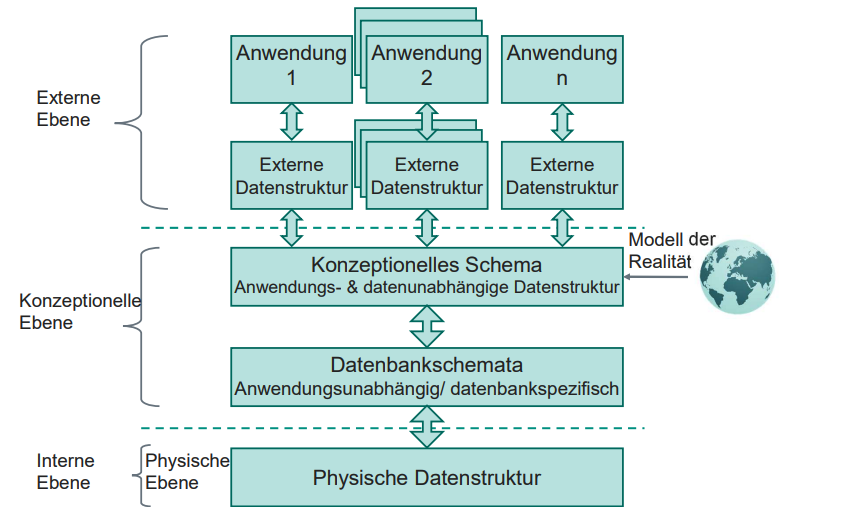
\includegraphics[width=\textwidth]{assets/images/ANSI3LayerModell}
    \caption{Aufbau des ANSI-3-Ebenen-Modells}
\end{figure}

Die ANSI-3-Ebenen-Architektur gibt es seit den 1970er-Jahren. \emph{ANSI} steht für \emph{American National Standards Institute} und ist damit in etwa mit dem deutschen DIN vergleichbar. Die 3-Ebenen-Architektur wird auch \emph{SPARC} genannt, abgeleitet von \emph{Standards Planning And Requirements Committee} -- einem Ausschuss innerhalb von ANSI, von dem die Architektur stammt.

\begin{merksatz}[ANSI/SPARC-Architektur]
Die 3-Sichten-Architektur ist die Grundlage einer konsistenten, modularen, interoperablen, wartbaren und skalierbaren Datenbank. Sie trennt die Daten in eine \textbf{interne}, eine \textbf{konzeptionelle} und eine \textbf{externe} Ebene.
\end{merksatz}

\subsubsection{Interne Ebene}
Die interne Ebene ist das Fundament einer Datenbank. Hier liegt ein Datenbankmodell zugrunde, wie es im Kapitel \emph{Datenbankmodelle} besprochen wird. Auf dieser Ebene werden die Aspekte der physischen Speicherung festgelegt -- also \emph{wie} und \emph{wo} die Daten konkret abgelegt werden.

\subsubsection{Konzeptionelle Ebene}
Die konzeptionelle Ebene ist das Bindeglied zwischen der internen und der externen Ebene. Hier werden die Daten modelliert, beispielsweise über ein ER-Diagramm. Auf dieser Ebene wird das Datenbankschema festgelegt, ebenso das konzeptionelle Schema für \icode{Primary Key}, \icode{Foreign Key} sowie sonstige Regeln zur Sicherung der Datenkonsistenz.

\subsubsection{Externe Ebene}
Die externe Ebene definiert, wie Nutzer auf die Datenbank zugreifen. Dazu zählen User Interfaces, Anwendungs-APIs, Views sowie -- im Fall einer API -- das Äquivalent in Form von \emph{Data Transfer Objects} (\icode{DTO}s). Hier können außerdem Plausibilitätsprüfungen und sonstige Integrationsregeln festgelegt werden. Auf dieser Ebene findet der \icode{SQL}-Zugriff statt.

\subsection{Datenbank-Entwurfsphasen}
\begin{figure}[H]
    \centering
    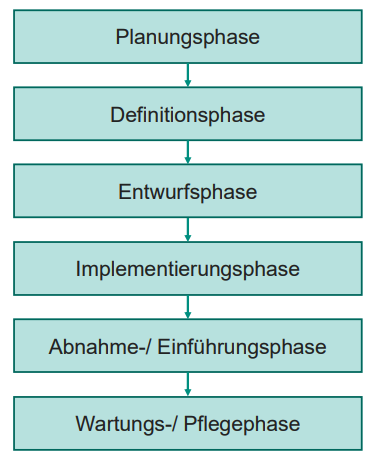
\includegraphics[width=\textwidth]{assets/images/DatenbankenPhase}
    \caption{Entwurfsphasen einer Datenbank}
\end{figure}
Der Entwurf einer Datenbank lässt sich in sechs Phasen unterteilen.

\subsubsection{Planungsphase}
In der Planungsphase geht es um die grundlegenden Festlegungen -- also darum, was überhaupt in der Datenbank gespeichert werden soll. Beispielsweise könnte ein Projekt darin bestehen, die Touren eines Logistikunternehmens zu speichern.

\subsubsection{Definitionsphase}
Hier wird festgelegt, welche Anforderungen die Datenbank erfüllen muss und welche Daten wo und wie erfasst werden müssen.

\subsubsection{Entwurfsphase}
Hier werden die technischen Entscheidungen getroffen -- etwa, welches Datenbankmodell genutzt wird. Außerdem entsteht in dieser Phase das ER-Diagramm.

\subsubsection{Implementierungsphase}
Hier wird der Entwurf in Code umgesetzt, meist als \icode{DDL} in \icode{SQL}. Eventuell werden auch Views angelegt und vielleicht sogar eine API.

\subsubsection{Abnahme- und Einführungsphase}
Hier werden die Datenbank bzw.\ die umgebende Software eingeführt. Anschließend wird geprüft, ob die Anwender mit der Anwendung zufrieden sind.

\subsubsection{Wartungs- und Pflegephase}
Hier werden mögliche Fehler behoben; auch eventuelle Erweiterungen fallen in diese Phase.